\chapter{Separación}%
\label{cha:separacion}

\section{Concepto}%
\label{sec:concepto}
\begin{defi}
Un espacio $X$ es \underline{Hausdorff} o $T_2$ si cada par de puntos distintos $x, y \in X$ tienen entornos disjuntos: $V^x \cap V^y = \emptyset$. 
\end{defi}
Hay otras formas de separación, más débiles o más fuertes, pero nos contentaremos con ésta al ser la más intuitiva.
\begin{obs}
\begin{enumerate}
    \item Si existen entornos disjuntos, existen entornos abiertos disjuntos [$\forall V \supset U$]
    \item Si $X$ es Hausdorff, los puntos son cerrados.
    \[
    \left[ \forall y \neq x, \exists U^y \not\ni x \Rightarrow X \setminus \{x\} = \bigcup_{y \neq x} U^y  \text{ es abierto.} \right] 
    \]
    \item $\left( X, \mathcal{T}_{CF} \right)$ no es Hausdorff: dos abiertos cualesquiera se cortan ($X$ infinito) tiene puntos cerrados: $X\setminus \{x\}$ es abierto.

    \item $\left( \mathbb{R}^n, \mathcal{T}_{u} \right)$ es Hausdorff: $x \neq y \Rightarrow B\left( x, \varepsilon \right) \cap B\left( y, \varepsilon \right) = \emptyset$ si $\varepsilon \le \lVert x - y \rVert / 2$

    \item En $\left( X, \mathcal{T}_a \right)$ el punto $a$ no es cerrado: $a \not\in X \setminus \{a\} \Rightarrow X \setminus \{a\}$ no es abierto. $\forall x \neq a \forall U^x \supset \{a, x\} \ni a$ !!!.
\end{enumerate}
\end{obs}

\begin{prop}
Sean $f, g: X \rightarrow Y$ continuas con $Y$ Hausdorff $\Rightarrow \{f = g\} = \{x \in X : f\left( x \right) = g\left( x \right)\}$ es cerrado.
\end{prop}
\begin{demo}
\begin{enumerate}
    \item $f\left( x \right) \neq g\left( x \right) \xRightarrow{T_2} \exists V^{f\left( x \right) \cap V\left( g\left( x \right) \right)} = \emptyset \xRightarrow{\text{cont.}} f^{-1}V^{f\left( x \right)} \cap g^{-1}V^{g\left( x \right)} = V^x$ entorno de $x$.

    \item $V^x \cap \{f = g\} = \emptyset: y \in V^x \Rightarrow \begin{cases}
        f\left( y \right) \in V^{f\left( x \right)} \\
        g\left( y \right) \in V^{g\left( x \right)} 
    \end{cases} \Rightarrow f\left( y \right) \neq g\left( y \right)$

    \item[1. + 2.] $X\setminus \{f = g\} = \{f \neq g\}$ es entorno de todos sus puntos, luego abierto, luego $\{f = g\}$ es cerrado.
\end{enumerate}
\end{demo}

\begin{coro}
Si $f = g$ es un subconjunto denso, entonces $f \equiv g$
\end{coro}
\begin{demo}
$\exists \overline{A} = X: f|_A = g|_A \Rightarrow \{f = g\} \supset A \xRightarrow{\text{prop.}} \{f = g\} \supset \overline{A} = X$.
\end{demo}

\underline{Caso particular importante}:
Funciones $f: X \rightarrow \mathbb{R}$.

\begin{obs}
$f: X \rightarrow \underbrace{Y}_{\in T_2}$ continua $\Rightarrow f^{-1}\left( Y \right)$ cerrado $\forall y \in Y$.

Porque  los puntos de $Y$ son cerrados y, de hecho, eso basta.
\end{obs}

\section{Tabla de comportamiento}%
\label{sec:tabla_de_comportamiento}
Se trata de saber si la propiedad se conserva por las construcciones conocidas.

Se tiene:
\begin{center}
\begin{tabular}{ c | c | c | c | c |}
    & Subespacios & Cocientes & Productos & Sumas\\
    \hline
    $T_2$ & \checkmark & $\times$ & \checkmark & \checkmark\\
    \hline
\end{tabular}
\end{center}
\begin{enumerate}
    \item $Y \subset X = T_2: y_1, y_2 \in Y \Rightarrow \exists \underbrace{V^{y_1}}_{\text{En } X}  \cap V^{y_2} = \emptyset \Rightarrow \underbrace{\left( V^{y_1} \cap Y \right)}_{\text{En } Y}  \cap \left( V^{y_2} \cap Y \right) = \emptyset$.

    \item $Y = \mathbb{R}/\mathbb{Q}: \begin{rcases}
        y_1 = \mathbb{Q} \in Y\\
        y_2 = \sqrt{2} \in Y
    \end{rcases} \nexists V^{y_1} \cap V^{y_2} = \emptyset: $ todo entorno abierto de $\sqrt{2}$ contiene racionales, luego al saturar, contiene $\mathbb{Q}$.

    \item $X$ y $Y$ ambos $T_2 \Leftrightarrow X \times Y$ $T_2$.

        $\Rightarrow)$
        \[
        \left( x_1, y_1 \right) \neq \left( x_2, y_2 \right) \in X \times Y \Rightarrow \begin{cases}
            x_1 \neq x_2 \Rightarrow \exists V^{x_1} \cap V^{x_2} = \emptyset \Rightarrow \left( V^{x_1} \times Y \right) \cap \left( V^{x_2} \times Y \right) = \emptyset
        \end{cases}  
        \]

        $\Leftarrow)$
        \[
        X \approx X \times \{y_0\} \subset X \times Y, T_2 \xRightarrow{1} X\times \{y_0\} T_2 \Rightarrow XT_2
        \]
        %TODO: Añadir texto
        \begin{figure}[H]
            \centering
            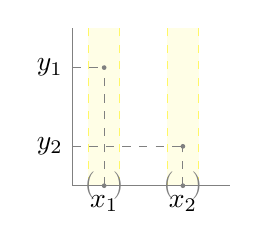
\begin{tikzpicture}
                \draw[-, gray] (0,0) -- (0,2);

                %Rectangulo izq
                \fill[fill=yellow!10, very thick, dashed] (0.2,2) rectangle (0.6,0);
                \draw[-, yellow!60] (0.2,0) -- (0.6,0);
                \draw[-, yellow!60, dashed] (0.2,0) -- (0.2,2);
                \draw[-, yellow!60, dashed] (0.6,0) -- (0.6,2);
                \fill[gray] (0.4,0) circle (0.03);

                %Rectangulo der
                \fill[fill=yellow!10, very thick, dashed] (1.2,2) rectangle (1.6,0);
                \draw[-, yellow!60] (1.2,0) -- (1.6,0);
                \draw[-, yellow!60, dashed] (1.2,0) -- (1.2,2);
                \draw[-, yellow!60, dashed] (1.6,0) -- (1.6,2);
                \fill[gray] (1.4,0) circle (0.03);

                \draw[-, gray] (0,0) -- (2,0) node[pos=0.11] {(}
                    node[pos=0.29] {)}
                    node[pos=0.61] {(}
                    node[pos=0.79] {)};
                postaction={decorate}

                \node(x1) at (0.4,0) [below] {$x_1$};
                \node(x2) at (1.4,0) [below] {$x_2$};

                \fill[gray] (0.4,1.5) circle (0.03);
                \fill[gray] (1.4,0.5) circle (0.03);

                \node(y1) at (0,1.5) [left] {$y_1$};
                \node(y2) at (0,0.5) [left] {$y_2$};

                %Lineas 1
                \draw[-, gray, dashed] (x1) -- (0.4,1.5);
                \draw[-, gray, dashed] (y1) -- (0.4,1.5);

                %Lineas 2
                \draw[-, gray, dashed] (x2) -- (1.4,0.5);
                \draw[-, gray, dashed] (y2) -- (1.4,0.5);
            \end{tikzpicture}
        \end{figure}

    \item $X$ y $Y$ ambos $T_2 \Leftrightarrow X + Y\ T_2$

    Único comentario: $x \in X$ y $y \in Y \Rightarrow X = V^x, Y = V^y$ y $X \cap Y = \emptyset$.
\end{enumerate}
